% Provenance (never printed): cycle 3 "Matiere, mouvement, energie,
% information" and "La planete Terre" (meteorological phenomena, the water in
% the air, measuring the weather); see sources/book1/PROVENANCE.md.
% Book 1, grade 4, chapter 1.
\chapter{Nuvens, chuva e neve}\label{ch:g4:clouds-rain-snow}

É uma tarde quente de verão. Na hora do almoço o céu estava azul, com
algumas nuvenzinhas brancas que pareciam bolas de algodão. Às três horas,
uma delas cresceu. Ela incha para cima, cada vez mais alto, como uma
couve-flor branca em pé sobre uma base cinzenta e achatada. O topo se
espalha. A base fica escura. Sopra uma rajada de vento fresco, caem as
primeiras gotas grossas e, durante vinte minutos, chove a cântaros. Depois
a \omterm{def:g4:clouds-rain-snow:cloud}{nuvem} vai embora, o sol volta e as calçadas molhadas soltam vapor.

De onde veio aquela \omterm{def:g4:clouds-rain-snow:cloud}{nuvem}? De que ela é feita? E quanta \omterm{def:g4:clouds-rain-snow:precipitation}{chuva} caiu
naqueles vinte minutos?

\begin{recall}
O \omterm{def:g1:watching-the-weather:weather}{tempo} é o estado do ar num certo lugar e num certo momento: ensolarado,
nublado, chuvoso, com \omterm{def:g4:clouds-rain-snow:precipitation}{neve}, com vento, com \omterm{def:g4:clouds-rain-snow:cloud}{neblina}; nós o anotamos num
\omterm{def:g1:watching-the-weather:weather-chart}{quadro do tempo} (\cref{ch:g1:watching-the-weather}). A água do \omterm{def:g2:water-on-earth:ocean}{mar}, dos
\omterm{def:g1:landscapes-around-us:water}{lagos} e do chão sobe para o ar e volta a cair como \omterm{def:g4:clouds-rain-snow:precipitation}{chuva}
(\cref{ch:g2:water-on-earth}). Os livros de física contam como a água
evapora (de líquido para um gás invisível), se condensa (de gás de volta
para gotinhas de líquido) e congela (de líquido para gelo), e como um
termômetro mede a temperatura em graus Celsius.
\end{recall}

\section{O que é uma nuvem?}

O ar à nossa volta sempre contém um pouco de água, em forma de um gás
invisível: o vapor de água. Quando o ar sobe, ele esfria. Quando esfria o
bastante, uma parte do vapor de água se condensa em gotículas de água tão
pequenas que o menor sopro de ar as mantém flutuando. Bilhões dessas
gotículas, lado a lado, formam uma \omterm{def:g4:clouds-rain-snow:cloud}{nuvem} que conseguimos ver. Lá no alto,
onde o ar é muito frio, as gotículas congelam, e a \omterm{def:g4:clouds-rain-snow:cloud}{nuvem} é feita de
pedacinhos minúsculos de gelo.

\begin{definition}[Nuvem e neblina]\label{def:g4:clouds-rain-snow:cloud}
Uma \emph{nuvem}\index{nuvem} é uma enorme quantidade de gotículas de água,
ou de pedacinhos minúsculos de gelo, flutuando juntos no ar. A
\emph{neblina}\index{neblina} é uma nuvem que encosta no chão.
\end{definition}

\begin{example}[A sua respiração numa manhã fria]\label{ex:g4:clouds-rain-snow:breath}
Numa manhã fria, a sua respiração forma uma nuvenzinha branca na frente
da sua boca. O ar que você solta é quente e contém vapor de água. O ar
frio o esfria na mesma hora, o vapor se condensa em gotículas minúsculas
--- e aparece uma \omterm{def:g4:clouds-rain-snow:cloud}{nuvem} em miniatura, que some quando as gotículas
evaporam de novo.
\end{example}

Uma \omterm{def:g4:clouds-rain-snow:cloud}{nuvem} é branca porque as suas gotículas espalham a luz do Sol em todas
as direções. Quando ela é muito espessa, pouca luz chega até a sua base, e
vista de baixo ela parece cinzenta, ou quase preta: é o sinal de uma \omterm{def:g4:clouds-rain-snow:cloud}{nuvem}
carregada, cheia de água.

\section{As famílias de nuvens}

As \omterm{def:g4:clouds-rain-snow:cloud}{nuvens} têm muitas formas, e os observadores do \omterm{def:g1:watching-the-weather:weather}{tempo} do mundo inteiro
as classificam do mesmo jeito: pela forma e pela altura em que flutuam.

\begin{definition}[Famílias de nuvens]\label{def:g4:clouds-rain-snow:cloud-families}
As quatro famílias de \omterm{def:g4:clouds-rain-snow:cloud}{nuvens} que é preciso conhecer são:
\begin{itemize}
  \item \emph{cúmulo}\index{cumulo@cúmulo}: \omterm{def:g4:clouds-rain-snow:cloud}{nuvens} amontoadas, brancas e fofas,
        com a base achatada, como bolas de algodão;
  \item \emph{estrato}\index{estrato}: \omterm{def:g4:clouds-rain-snow:cloud}{nuvens} em camada, uma lâmina cinzenta
        e plana que cobre o céu inteiro, lá embaixo;
  \item \emph{cirro}\index{cirro}: \omterm{def:g4:clouds-rain-snow:cloud}{nuvens} em fiapos, fios brancos e finos ou
        cachos, muito altas, feitas de gelo;
  \item \emph{cumulonimbo}\index{cumulonimbo}: a \omterm{def:g4:clouds-rain-snow:cloud}{nuvem} de tempestade, uma
        torre enorme que sobe de uma base baixa e escura até uma altura
        muito grande, e cujo topo muitas vezes se espalha, achatado.
\end{itemize}
\end{definition}

Os nomes vêm de palavras latinas: \emph{cumulus} quer dizer monte,
\emph{stratus} camada, \emph{cirrus} cacho de cabelo e \emph{nimbus} \omterm{def:g4:clouds-rain-snow:cloud}{nuvem} de \omterm{def:g4:clouds-rain-snow:precipitation}{chuva}.

\begin{omfigure}
\begin{minipage}[b]{0.49\linewidth}\centering
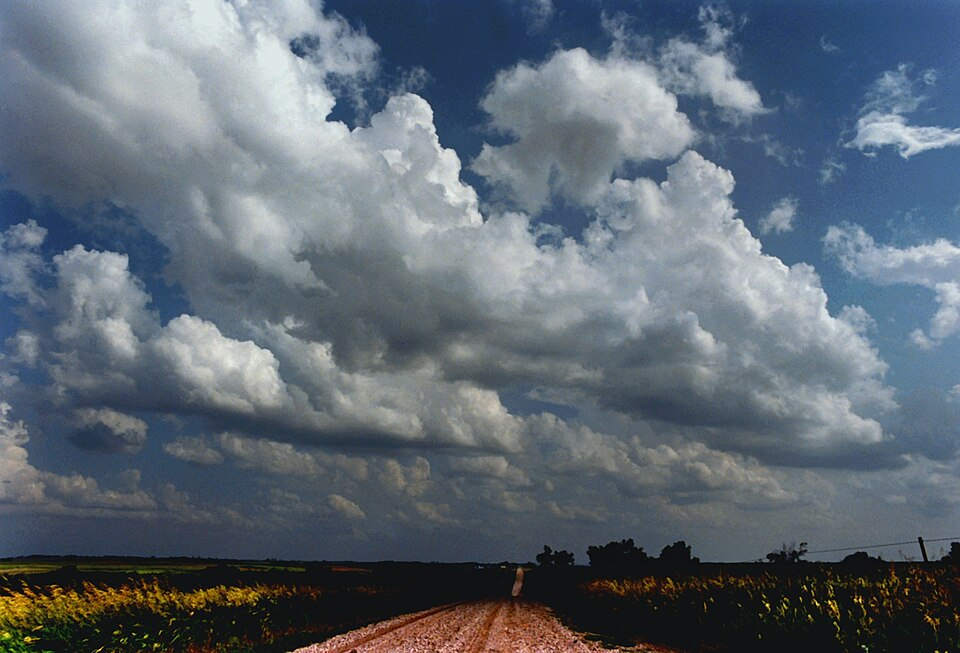
\includegraphics[width=\linewidth]{images/book1/g4-cumulus.jpg}

{\small \omterm{def:g4:clouds-rain-snow:cloud-families}{Cúmulos}, \omterm{def:g4:clouds-rain-snow:cloud}{nuvens} amontoadas de base achatada.}
\end{minipage}\hfill
\begin{minipage}[b]{0.49\linewidth}\centering
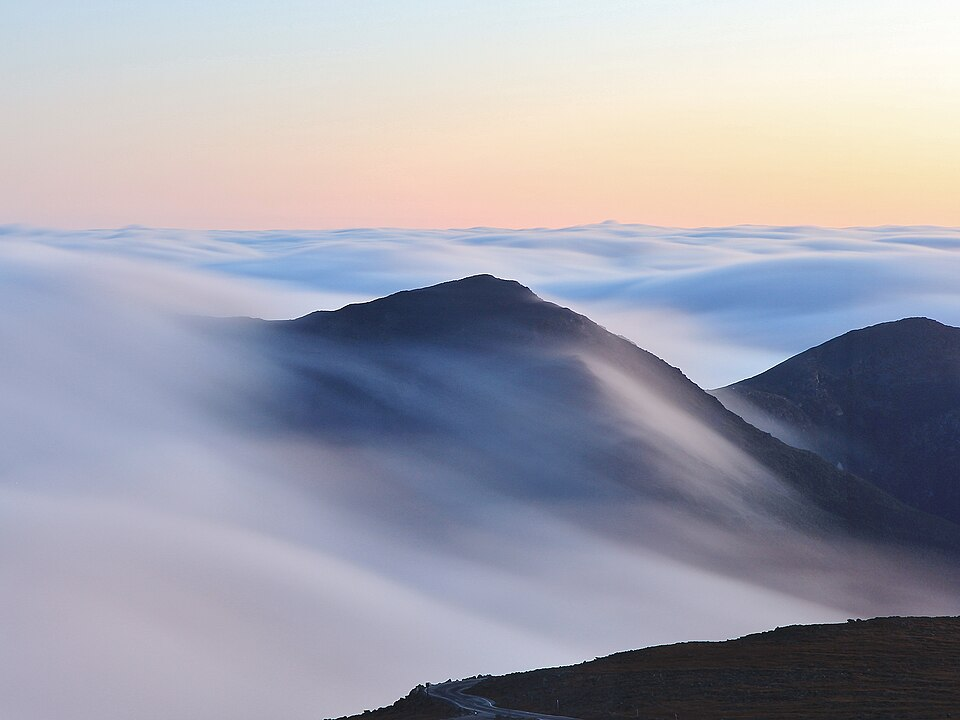
\includegraphics[width=\linewidth]{images/book1/g4-stratus.jpg}

{\small \omterm{def:g4:clouds-rain-snow:cloud-families}{Estratos}: uma camada plana, vista aqui de cima, de uma \omterm{def:g1:landscapes-around-us:landform}{montanha}.}
\end{minipage}

\medskip
\begin{minipage}[b]{0.49\linewidth}\centering
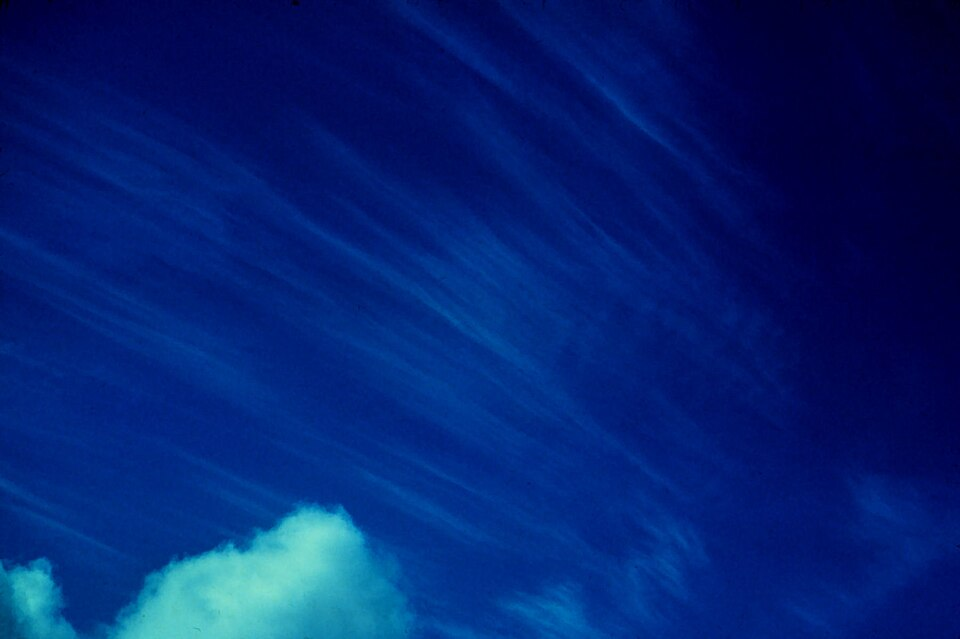
\includegraphics[width=\linewidth]{images/book1/g4-cirrus.jpg}

{\small \omterm{def:g4:clouds-rain-snow:cloud-families}{Cirros}: fios finos de gelo, muito altos (com um pequeno \omterm{def:g4:clouds-rain-snow:cloud-families}{cúmulo} embaixo).}
\end{minipage}\hfill
\begin{minipage}[b]{0.49\linewidth}\centering
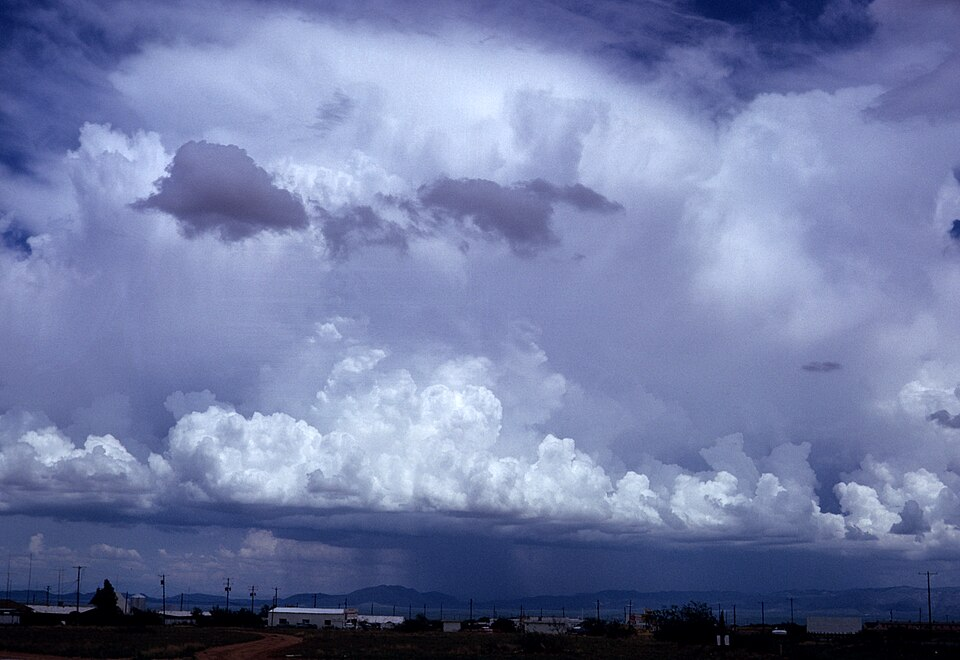
\includegraphics[width=\linewidth]{images/book1/g4-cumulonimbus.jpg}

{\small Um \omterm{def:g4:clouds-rain-snow:cloud-families}{cumulonimbo}: uma torre de \omterm{def:g4:clouds-rain-snow:cloud}{nuvem}; a \omterm{def:g4:clouds-rain-snow:precipitation}{chuva} cai da sua base escura.}
\end{minipage}

\smallskip
{\small Fotos: NOAA Photo Library (domínio público): S. Corfidi
(\omterm{def:g4:clouds-rain-snow:cloud-families}{cúmulos}), R. F. Kresge (\omterm{def:g4:clouds-rain-snow:cloud-families}{cirros}), coleção B. Hooke (\omterm{def:g4:clouds-rain-snow:cloud-families}{cumulonimbo}).}
% ledger: noaa:photos-g4
\label{fig:g4:clouds-rain-snow:photos}
\end{omfigure}

A que altura flutuam as \omterm{def:g4:clouds-rain-snow:cloud}{nuvens}? Depende da família. As \omterm{def:g4:clouds-rain-snow:cloud}{nuvens} baixas, como
os \omterm{def:g4:clouds-rain-snow:cloud-families}{estratos} e a base dos \omterm{def:g4:clouds-rain-snow:cloud-families}{cúmulos}, flutuam desde pouco acima do chão até
cerca de 2 quilômetros. Os \omterm{def:g4:clouds-rain-snow:cloud-families}{cirros} flutuam muito alto, entre cerca de 5 e 13
quilômetros fora dos trópicos e das regiões polares --- muitas vezes mais
alto que a \omterm{def:g1:landscapes-around-us:landform}{montanha} mais alta da Terra.
Um \omterm{def:g4:clouds-rain-snow:cloud-families}{cumulonimbo} se estende desde uma base baixa até o topo dos níveis de
\omterm{def:g4:clouds-rain-snow:cloud}{nuvens}.
% ledger: wmo:cloud-levels, wmo:cumulonimbus

\begin{omfigure}
\begin{tikzpicture}[x=1cm, y=0.5cm, font=\small]
  % height scale
  \draw[black!60] (0,0) -- (0,14);
  \foreach \h in {0,2,...,14} {
    \draw[black!60] (-0.1,\h) -- (0,\h);
    \node[anchor=east, font=\scriptsize] at (-0.12,\h) {\h\,km};
  }
  \node[anchor=south, font=\scriptsize, align=center] at (0,14.2) {altura};
  % ground and a mountain for comparison
  \fill[green!35!black!50] (0.2,0) -- (11.4,0) -- (11.4,-0.4) -- (0.2,-0.4) -- cycle;
  \fill[black!35] (8.6,0) -- (9.9,8.8) -- (10.2,8.4) -- (11.2,0) -- cycle;
  \fill[white, draw=black!45, line width=0.3pt] (9.65,7.2) -- (9.9,8.8) -- (10.2,8.4) -- (10.4,7.0) -- (10.1,7.4) -- (9.9,7.0) -- cycle;
  \node[font=\scriptsize, align=center] at (9.9,10.2) {a montanha\\mais alta};
  % levels
  \fill[blue!6] (0.2,0.15) rectangle (8.3,2);
  \fill[blue!10] (0.2,5) rectangle (8.3,13);
  \node[anchor=west, font=\scriptsize, text=blue!50!black] at (0.3,1.65) {nuvens baixas};
  \node[anchor=west, font=\scriptsize, text=blue!50!black] at (0.3,12.6) {nuvens altas};
  % stratus: a flat grey layer
  \fill[black!25, rounded corners=2pt] (0.6,0.6) rectangle (2.6,1.3);
  \node[font=\scriptsize] at (1.6,-1.1) {estrato};
  % cumulus
  \pic[scale=0.7, transform shape] at (4.0,0.9) {puffycloud};
  \node[font=\scriptsize] at (4.0,-1.1) {cúmulo};
  % cirrus: wisps
  \foreach \y in {9.4,10.0,10.6} {
    \draw[black!50, line width=0.6pt] (0.8,\y) .. controls (1.4,\y+0.5) and (2.0,\y+0.1) .. (2.6,\y+0.6);
  }
  \node[font=\scriptsize] at (1.7,8.5) {cirro};
  % cumulonimbus: tower with an anvil
  \fill[black!15, draw=black!45, line width=0.4pt]
    (5.4,1.0) .. controls (5.2,4) and (5.6,8) .. (5.9,11.2)
    .. controls (5.0,11.6) and (4.6,12.0) .. (4.8,12.3)
    -- (8.1,12.3) .. controls (8.2,12.0) and (7.8,11.6) .. (7.0,11.2)
    .. controls (7.3,8) and (7.6,4) .. (7.4,1.0) -- cycle;
  \fill[black!45] (5.4,1.0) rectangle (7.4,1.4);
  \foreach \x in {5.7,6.1,6.5,6.9,7.2}
    \draw[omWxRain, line width=0.6pt] (\x,0.95) -- (\x-0.15,0.15);
  \node[font=\scriptsize] at (6.4,-1.1) {cumulonimbo};
\end{tikzpicture}

{\small A que altura flutuam as quatro famílias de \omterm{def:g4:clouds-rain-snow:cloud}{nuvens} (alturas em
quilômetros, para regiões que não são nem tropicais nem polares). O
\omterm{def:g4:clouds-rain-snow:cloud-families}{estrato} e a base do \omterm{def:g4:clouds-rain-snow:cloud-families}{cúmulo} são baixos; os \omterm{def:g4:clouds-rain-snow:cloud-families}{cirros} muitas vezes ficam mais
altos que a \omterm{def:g1:landscapes-around-us:landform}{montanha} mais alta. Um \omterm{def:g4:clouds-rain-snow:cloud-families}{cumulonimbo} se estende de uma base
baixa até o topo dos níveis de \omterm{def:g4:clouds-rain-snow:cloud}{nuvens}. Alturas segundo o atlas de \omterm{def:g4:clouds-rain-snow:cloud}{nuvens}
da Organização Meteorológica Mundial.}
\label{fig:g4:clouds-rain-snow:heights}
% ledger: wmo:cloud-levels, tht:everest
\end{omfigure}

\begin{method}[Dar nome a uma nuvem]\label{met:g4:clouds-rain-snow:naming}
Olhe o céu e faça três perguntas:
\begin{enumerate}
  \item É um monte de base achatada? Então é um \omterm{def:g4:clouds-rain-snow:cloud-families}{cúmulo} --- e, se ele
        sobe e vira uma torre enorme e escura, um \omterm{def:g4:clouds-rain-snow:cloud-families}{cumulonimbo}.
  \item É uma lâmina plana e uniforme que esconde o céu inteiro? Então é
        um \omterm{def:g4:clouds-rain-snow:cloud-families}{estrato}.
  \item É feita de fios brancos e finos, muito altos? Então é um \omterm{def:g4:clouds-rain-snow:cloud-families}{cirro}.
\end{enumerate}
\end{method}

\begin{remark}[As nuvens anunciam o tempo]\label{rem:g4:clouds-rain-snow:tell}
\omterm{def:g4:clouds-rain-snow:cloud-families}{Cúmulos} pequenos num céu azul significam \omterm{def:g1:watching-the-weather:weather}{tempo} bom. Um \omterm{def:g4:clouds-rain-snow:cloud-families}{estrato} cinzento
traz um dia fechado, às vezes com garoa. Um \omterm{def:g4:clouds-rain-snow:cloud-families}{cumulonimbo} traz uma pancada
de \omterm{def:g4:clouds-rain-snow:precipitation}{chuva} curta e forte, muitas vezes com trovões, raios e rajadas de vento
--- às vezes \omterm{def:g4:clouds-rain-snow:precipitation}{granizo}. Os \omterm{def:g4:clouds-rain-snow:cloud-families}{cirros} não trazem \omterm{def:g4:clouds-rain-snow:precipitation}{chuva}, mas, quando se espalham e
ficam mais espessos, muitas vezes chove um dia depois.
\end{remark}

\section{Chuva, neve e granizo}

Dentro de uma \omterm{def:g4:clouds-rain-snow:cloud}{nuvem}, as gotículas minúsculas se chocam e se juntam, ou
cristais de gelo crescem à custa das gotículas. Uma gota de \omterm{def:g4:clouds-rain-snow:cloud}{nuvem}, ou um
cristal, que ficou grande e pesado o bastante não consegue mais flutuar: ele cai.

\begin{definition}[Precipitação]\label{def:g4:clouds-rain-snow:precipitation}
A \emph{precipitação}\index{precipitacao@precipitação} é a água que cai de uma \omterm{def:g4:clouds-rain-snow:cloud}{nuvem}
até o chão: \emph{chuva}\index{chuva} (gotas de água líquida),
\emph{neve}\index{neve} (flocos feitos de cristais de gelo grudados) ou
\emph{granizo}\index{granizo} (bolas de gelo, chamadas pedras de granizo,
que caem das \omterm{def:g4:clouds-rain-snow:cloud}{nuvens} de tempestade).
\end{definition}

Se vai chover ou nevar depende da temperatura do ar que a \omterm{def:g4:clouds-rain-snow:precipitation}{precipitação}
atravessa. Os flocos de \omterm{def:g4:clouds-rain-snow:precipitation}{neve} se formam no alto da \omterm{def:g4:clouds-rain-snow:cloud}{nuvem} fria. Se o ar mais
embaixo estiver acima de \SI{0}{\celsius} por tempo suficiente, eles
derretem no caminho e chegam até nós como \omterm{def:g4:clouds-rain-snow:precipitation}{chuva}. Se o ar estiver abaixo de
zero até o chão, eles chegam como \omterm{def:g4:clouds-rain-snow:precipitation}{neve}.

\begin{omfigure}

\includegraphics[width=0.55\linewidth]{images/book1/ai/g4-snowflakes.jpg}

{\small Crianças pegando flocos de \omterm{def:g4:clouds-rain-snow:precipitation}{neve} numa luva escura: cada floco é feito
de cristais de gelo.}
\end{omfigure}

O \omterm{def:g4:clouds-rain-snow:precipitation}{granizo} só cai dos \omterm{def:g4:clouds-rain-snow:cloud-families}{cumulonimbos}. Dentro da torre, ventos fortes que sobem
levam bolinhas de gelo para cima e para baixo várias vezes; cada viagem
acrescenta uma nova camada de gelo, como as camadas de uma cebola, até a
pedra de \omterm{def:g4:clouds-rain-snow:precipitation}{granizo} ficar pesada demais para o vento segurá-la.

\begin{omfigure}
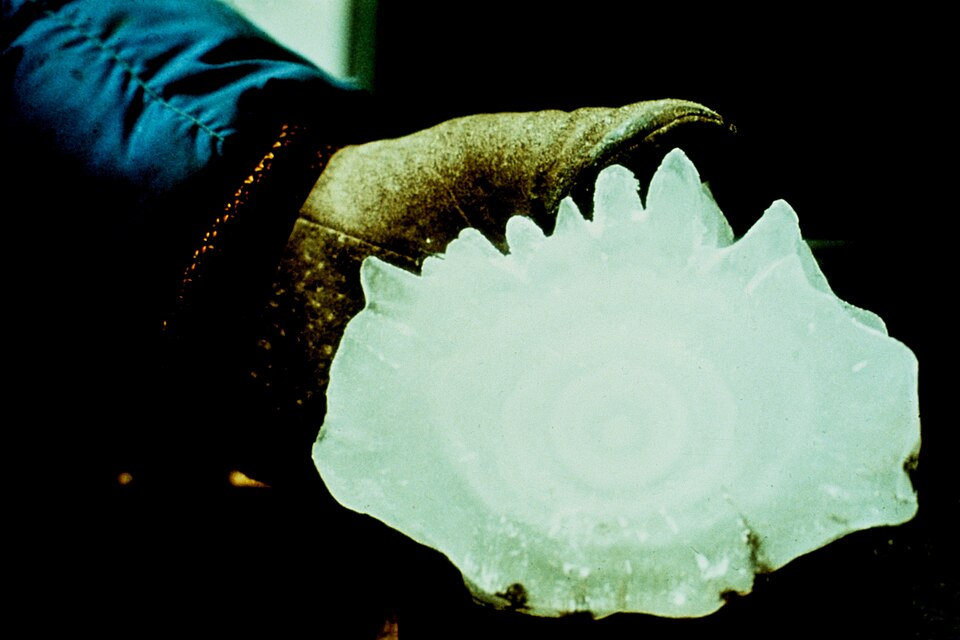
\includegraphics[width=0.5\linewidth]{images/book1/g4-hailstone.jpg}

{\small Uma pedra de \omterm{def:g4:clouds-rain-snow:precipitation}{granizo} muito grande na mão de alguém de luva. Os anéis
mostram as camadas de gelo que ela juntou dentro da \omterm{def:g4:clouds-rain-snow:cloud}{nuvem} de tempestade.
Foto: NOAA Photo Library (domínio público).}
% ledger: noaa:photos-g4
\end{omfigure}

\section{Medir o tempo}

Para dizer quanto choveu, qual era a temperatura ou de onde soprava o
vento, palavras não bastam: precisamos de instrumentos, e de números.

\begin{definition}[Pluviômetro]\label{def:g4:clouds-rain-snow:rain-gauge}
Um \emph{pluviômetro}\index{pluviometro@pluviômetro} é um recipiente que recolhe a
\omterm{def:g4:clouds-rain-snow:precipitation}{chuva} que cai na sua abertura. A altura da água recolhida é medida em
milímetros: ``5 milímetros de \omterm{def:g4:clouds-rain-snow:precipitation}{chuva}'' quer dizer que a \omterm{def:g4:clouds-rain-snow:precipitation}{chuva} teria formado
uma camada de água de 5 milímetros de altura sobre um chão plano, se nada
tivesse escorrido nem se infiltrado.
\end{definition}

\begin{remark}[Um milímetro de chuva é muita água]\label{rem:g4:clouds-rain-snow:litre}
Um milímetro de \omterm{def:g4:clouds-rain-snow:precipitation}{chuva} parece pouquinho no \omterm{def:g4:clouds-rain-snow:rain-gauge}{pluviômetro}. Mas, num quadrado de
chão de um metro por um metro, isso dá um litro de água: uma garrafa
grande. Num pátio de escola de mil metros quadrados, uma \omterm{def:g4:clouds-rain-snow:precipitation}{chuva} de 10
milímetros traz dez mil litros: o suficiente para encher mil baldes de 10
litros cada um.
\end{remark}

\begin{omfigure}
\begin{tikzpicture}[font=\small]
  % funnel
  \draw[black!70, line width=0.8pt] (-1.2,6.6) -- (-0.35,5.8) -- (-0.35,5.4);
  \draw[black!70, line width=0.8pt] (1.2,6.6) -- (0.35,5.8) -- (0.35,5.4);
  \draw[black!70, line width=0.8pt] (-1.2,6.6) -- (1.2,6.6);
  % tube
  \fill[blue!25] (-0.45,0) rectangle (0.45,2.4);
  \draw[black!70, line width=0.8pt] (-0.45,5.4) -- (-0.45,0) -- (0.45,0) -- (0.45,5.4);
  \foreach \m in {0,1,...,50} {
    \pgfmathsetmacro{\yy}{\m*0.1}
    \draw[black!60] (0.45,\yy) -- ++(-0.12,0);
  }
  \foreach \m in {0,5,10,...,50} {
    \pgfmathsetmacro{\yy}{\m*0.1}
    \draw[black!80] (0.45,\yy) -- ++(-0.25,0);
    \node[anchor=west, font=\scriptsize] at (0.5,\yy) {\m};
  }
  \node[anchor=west, font=\scriptsize] at (1.0,5.0) {mm};
  % reading line
  \draw[red!70!black, -{Stealth}] (-1.6,2.4) -- (-0.5,2.4);
  \node[anchor=east, align=right, font=\scriptsize] at (-1.65,2.4) {leia o\\nível aqui};
  \node[anchor=west, font=\scriptsize] at (1.9,2.4) {$\leftarrow$ 24\,mm de chuva};
\end{tikzpicture}

{\small Um \omterm{def:g4:clouds-rain-snow:rain-gauge}{pluviômetro} simples: um funil recolhe a \omterm{def:g4:clouds-rain-snow:precipitation}{chuva} e um tubo
graduado em milímetros a guarda. Leia o nível da água com o olho na mesma
altura. Aqui, caíram 24 milímetros desde a última vez em que o
\omterm{def:g4:clouds-rain-snow:rain-gauge}{pluviômetro} foi esvaziado.}
\label{fig:g4:clouds-rain-snow:gauge}
\end{omfigure}


\begin{definition}[Cata-vento]\label{def:g4:clouds-rain-snow:wind-vane}
Um \emph{cata-vento}\index{cata-vento} é uma seta que gira livremente num
mastro. O vento empurra a cauda dela; por isso a seta sempre aponta para
a direção \emph{de onde} o vento vem.
\end{definition}

\begin{definition}[Estação meteorológica]\label{def:g4:clouds-rain-snow:weather-station}
Uma \emph{estação meteorológica}\index{estacao meteorologica@estação meteorológica} é um lugar onde o \omterm{def:g1:watching-the-weather:weather}{tempo}
é medido todos os dias, sempre do mesmo jeito, com instrumentos: um
termômetro num abrigo branco ventilado, um \omterm{def:g4:clouds-rain-snow:rain-gauge}{pluviômetro} ao ar livre, um
\omterm{def:g4:clouds-rain-snow:wind-vane}{cata-vento} num mastro.
\end{definition}

O termômetro fica na sombra, num abrigo branco com laterais de venezianas,
que deixam o ar passar mas não deixam entrar o sol nem a \omterm{def:g4:clouds-rain-snow:precipitation}{chuva}. O Met
Office, o serviço meteorológico do Reino Unido, o coloca a
\SI{1.25}{\metre} do chão. O \omterm{def:g4:clouds-rain-snow:rain-gauge}{pluviômetro} fica ao ar livre, longe de muros
e de árvores que o protegeriam da \omterm{def:g4:clouds-rain-snow:precipitation}{chuva}, com a abertura um pouco acima do
chão. O \omterm{def:g4:clouds-rain-snow:wind-vane}{cata-vento} fica bem no alto do seu mastro, acima dos obstáculos
que desviariam o vento.
% ledger: mo:screen-height, mo:raingauge

\begin{omfigure}
\begin{tikzpicture}[font=\small, x=1cm, y=1cm]
  % grass
  \fill[green!40!black!45] (-0.5,0) rectangle (11,-0.25);
  \foreach \x in {-0.3,0.1,...,10.8} \draw[green!45!black] (\x,0) -- ++(0.06,0.14);
  % screen on legs
  \draw[black!70, line width=1pt] (0.8,0) -- (0.8,1.25) (2.2,0) -- (2.2,1.25);
  \fill[white, draw=black!70] (0.6,1.25) rectangle (2.4,2.4);
  \foreach \y in {1.4,1.55,...,2.25} \draw[black!40] (0.7,\y) -- (2.3,\y-0.08);
  \fill[white, draw=black!70] (0.45,2.4) -- (1.5,2.75) -- (2.55,2.4) -- cycle;
  \draw[black!60, <->] (2.8,0) -- node[right, font=\scriptsize, align=left] {cerca de\\1.25\,m} (2.8,1.25);
  \node[align=center, font=\scriptsize] at (1.5,3.25) {termômetro num\\abrigo de venezianas};
  % rain gauge
  \fill[black!15, draw=black!70] (5.4,0) rectangle (5.9,0.4);
  \draw[black!70] (5.3,0.55) -- (5.4,0.4) (6.0,0.55) -- (5.9,0.4);
  \node[align=center, font=\scriptsize] at (5.65,1.2) {pluviômetro,\\ao ar livre};
  % tree far away
  \fill[brown!60!black] (7.3,0) rectangle (7.5,1.3);
  \fill[green!50!black!70] (7.4,2.1) circle (0.85);
  % wind vane on a mast
  \draw[black!70, line width=1pt] (9.8,0) -- (9.8,4.2);
  \draw[black!80, line width=1.4pt, -{Latex[length=3mm]}] (10.6,4.4) -- (9.0,4.4);
  \fill[black!80] (10.6,4.4) -- (10.9,4.65) -- (10.9,4.15) -- cycle;
  \node[align=center, font=\scriptsize] at (9.8,5.05) {cata-vento num mastro alto};
  \node[anchor=west, font=\scriptsize, align=left] at (10.1,3.4) {aponta para onde\\o vento vem};
\end{tikzpicture}

{\small Uma pequena \omterm{def:g4:clouds-rain-snow:weather-station}{estação meteorológica}. O termômetro fica na sombra, num
abrigo branco com laterais de venezianas, a cerca de 1.25 metro acima da
grama; o \omterm{def:g4:clouds-rain-snow:rain-gauge}{pluviômetro} fica ao ar livre, longe da árvore; o \omterm{def:g4:clouds-rain-snow:wind-vane}{cata-vento} fica
bem acima dos obstáculos.}
\label{fig:g4:clouds-rain-snow:station}
% ledger: mo:screen-height
\end{omfigure}

\begin{inthefield}[Uma estação meteorológica no pátio da escola]
Muitas escolas mantêm uma pequena \omterm{def:g4:clouds-rain-snow:weather-station}{estação meteorológica} num canto do
pátio. Toda manhã, no mesmo horário, dois alunos leem o termômetro, leem e
esvaziam o \omterm{def:g4:clouds-rain-snow:rain-gauge}{pluviômetro} e anotam para onde o \omterm{def:g4:clouds-rain-snow:wind-vane}{cata-vento} aponta. Com o passar
das semanas, a turma monta um registro do seu próprio \omterm{def:g1:watching-the-weather:weather}{tempo}.
\end{inthefield}

\begin{omfigure}
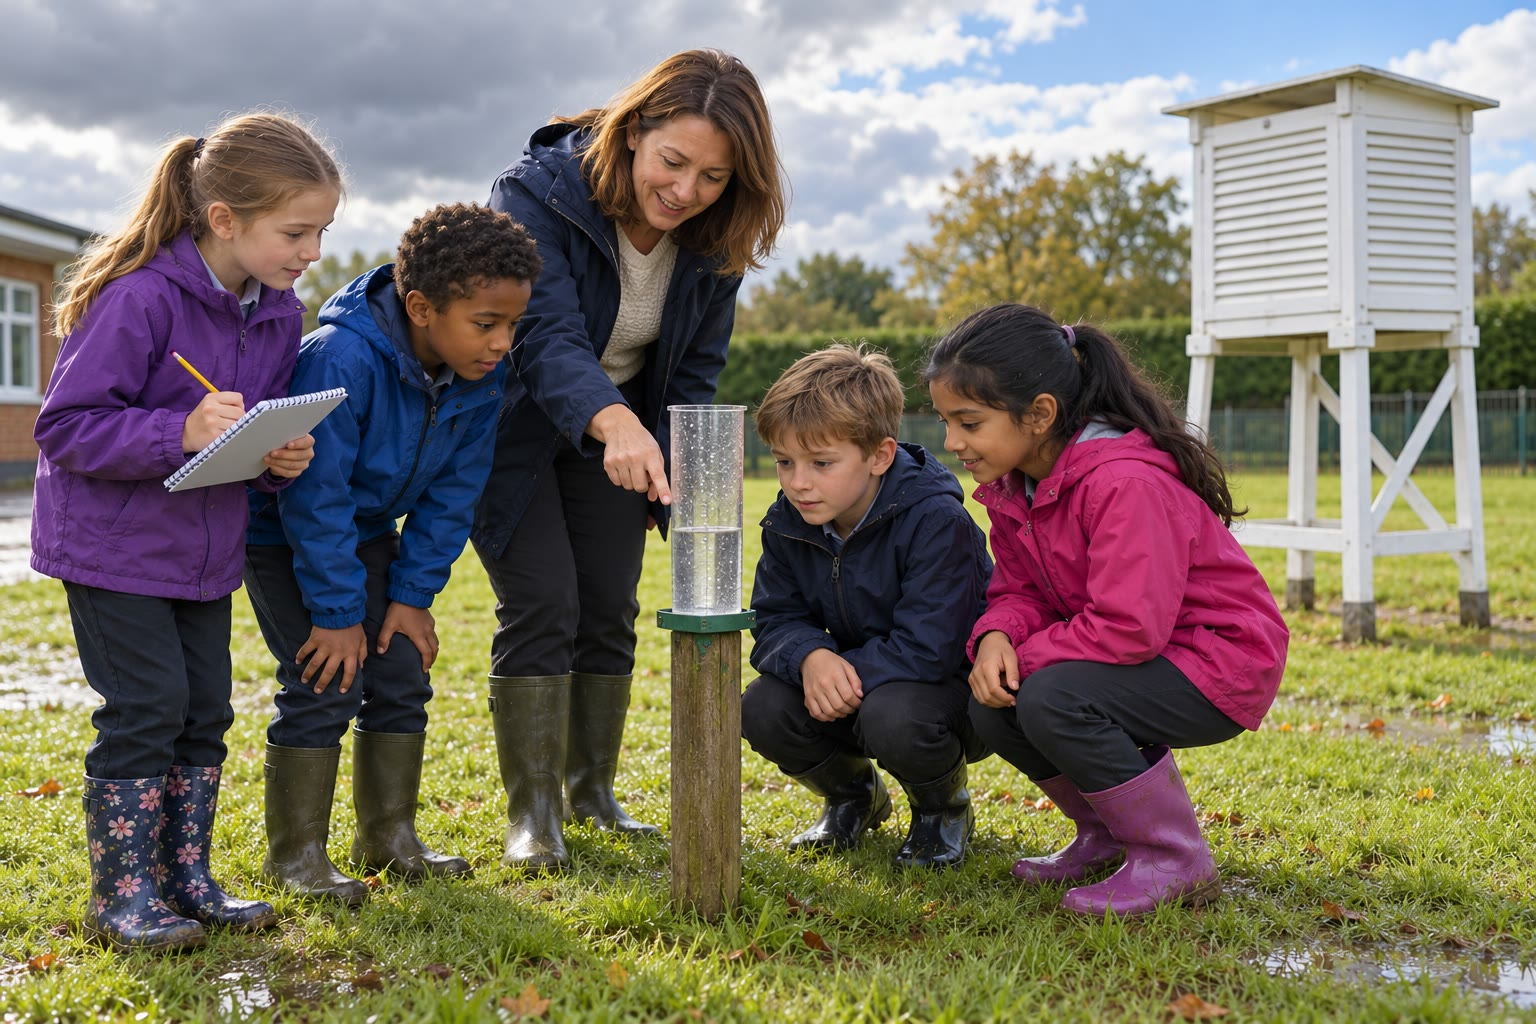
\includegraphics[width=0.55\linewidth]{images/book1/ai/g4-rain-gauge-class.jpg}

{\small Alunos lendo o \omterm{def:g4:clouds-rain-snow:rain-gauge}{pluviômetro} no pátio da escola.}
\end{omfigure}

\begin{method}[Desenhar um gráfico de barras da chuva]\label{met:g4:clouds-rain-snow:bar-chart}
Para desenhar a \omterm{def:g4:clouds-rain-snow:precipitation}{chuva} de uma semana:
\begin{enumerate}
  \item trace uma linha horizontal e escreva os dias embaixo dela, com o
        mesmo espaço entre eles;
  \item trace uma linha vertical à esquerda e marque-a em milímetros, com
        passos iguais (por exemplo, de 2 em 2 milímetros);
  \item acima de cada dia, desenhe uma barra da altura da \omterm{def:g4:clouds-rain-snow:precipitation}{chuva} desse dia;
        um dia sem \omterm{def:g4:clouds-rain-snow:precipitation}{chuva} não tem barra nenhuma;
  \item dê um título ao gráfico e escreva a unidade, mm, na linha vertical.
\end{enumerate}
\end{method}

\begin{example}[Uma semana de chuva na escola]\label{ex:g4:clouds-rain-snow:week}
A turma leu o \omterm{def:g4:clouds-rain-snow:rain-gauge}{pluviômetro} toda manhã durante uma semana e encontrou:
segunda 0, terça 4, quarta 12, quinta 7, sexta 0, sábado 2, domingo 5
milímetros. O dia mais chuvoso foi a quarta-feira. Não choveu na segunda
nem na sexta. Na semana inteira caíram $0 + 4 + 12 + 7 + 0 + 2 + 5 = 30$
milímetros. Só a quarta-feira trouxe 12 dos 30 milímetros, ou seja,
$\frac{12}{30} = \frac{2}{5}$ da \omterm{def:g4:clouds-rain-snow:precipitation}{chuva} da semana.
\end{example}

\begin{omfigure}
\begin{tikzpicture}
\begin{axis}[ybar, bar width=14pt, width=0.8\linewidth, height=5.4cm,
    ymin=0, ymax=14, ytick={0,2,...,14}, ylabel={chuva (mm)},
    symbolic x coords={Mon,Tue,Wed,Thu,Fri,Sat,Sun}, xtick=data,
    xticklabels={seg,ter,qua,qui,sex,sáb,dom},
    axis x line*=bottom, axis y line*=left, ymajorgrids, grid style={gray!25},
    nodes near coords, nodes near coords style={font=\scriptsize},
    every axis label/.append style={font=\small}, tick label style={font=\small},
    title={Chuva na escola durante uma semana}, title style={font=\small}]
  \addplot[fill=omWxRain!70, draw=omWxRain!60!black] coordinates
    {(Mon,0) (Tue,4) (Wed,12) (Thu,7) (Fri,0) (Sat,2) (Sun,5)};
\end{axis}
\end{tikzpicture}

{\small A semana do \cref{ex:g4:clouds-rain-snow:week} num gráfico de barras.}
\label{fig:g4:clouds-rain-snow:bars}
\end{omfigure}

\section{Exercícios}

\begin{exercise}[$\star$]\label{exo:g4:clouds-rain-snow:1}
De que é feita uma \omterm{def:g4:clouds-rain-snow:cloud}{nuvem}? O que é a \omterm{def:g4:clouds-rain-snow:cloud}{neblina}?
\end{exercise}

\begin{exercise}[$\star$]\label{exo:g4:clouds-rain-snow:2}
Dê o nome da \omterm{def:g4:clouds-rain-snow:cloud}{nuvem}: (a) uma lâmina cinzenta e plana que esconde o céu
inteiro; (b) fios brancos e finos muito altos num céu azul; (c) montes
brancos de base achatada, como algodão; (d) uma torre enorme e escura de
topo achatado, que traz trovões.
\end{exercise}

\begin{exercise}[$\star$]\label{exo:g4:clouds-rain-snow:3}
\omterm{def:g4:clouds-rain-snow:precipitation}{Chuva}, \omterm{def:g4:clouds-rain-snow:precipitation}{neve} ou \omterm{def:g4:clouds-rain-snow:precipitation}{granizo}? (a) bolas de gelo que caem de uma \omterm{def:g4:clouds-rain-snow:cloud}{nuvem} de
tempestade; (b) gotas de água líquida; (c) flocos feitos de cristais de gelo.
\end{exercise}

\begin{exercise}[$\star$]\label{exo:g4:clouds-rain-snow:4}
Que instrumento mede: (a) a \omterm{def:g4:clouds-rain-snow:precipitation}{chuva}; (b) a temperatura; (c) de onde vem o
vento?
\end{exercise}

\begin{exercise}[$\star$]\label{exo:g4:clouds-rain-snow:5}
No \omterm{def:g4:clouds-rain-snow:rain-gauge}{pluviômetro} desenhado na página~\pageref{fig:g4:clouds-rain-snow:gauge}, a água
agora chega à marca 17. Quantos milímetros de \omterm{def:g4:clouds-rain-snow:precipitation}{chuva} caíram? Quantos
milímetros a mais a levariam até 20?
\end{exercise}

\begin{exercise}[$\star$]\label{exo:g4:clouds-rain-snow:6}
Observe o gráfico de barras da página~\pageref{fig:g4:clouds-rain-snow:bars}. Qual
foi o dia mais chuvoso? Em que dias não choveu? Que dia teve 7
milímetros?
\end{exercise}

\begin{exercise}[$\star\star$]\label{exo:g4:clouds-rain-snow:7}
Na manhã de um dia de \omterm{def:g4:clouds-rain-snow:precipitation}{neve}, os flocos chegam ao chão na vila da \omterm{def:g1:landscapes-around-us:landform}{montanha},
mas no \omterm{def:g1:landscapes-around-us:landform}{vale} lá embaixo chove. Explique a diferença usando a temperatura
do ar.
\end{exercise}

\begin{exercise}[$\star\star$]\label{exo:g4:clouds-rain-snow:8}
Em outra semana, a turma encontra: segunda 3, terça 0, quarta 1, quinta 9,
sexta 6, sábado 0, domingo 1 milímetro. Desenhe o gráfico de barras.
Quantos milímetros caíram na semana? Que fração da \omterm{def:g4:clouds-rain-snow:precipitation}{chuva} da semana caiu
na quinta-feira?
\end{exercise}

\begin{exercise}[$\star\star$]\label{exo:g4:clouds-rain-snow:9}
Por que o \omterm{def:g4:clouds-rain-snow:rain-gauge}{pluviômetro} tem de ficar ao ar livre, longe de muros e de
árvores? Por que o termômetro fica num abrigo branco na sombra, e não em
pleno sol?
\end{exercise}

\begin{exercise}[$\star\star$]\label{exo:g4:clouds-rain-snow:10}
O \omterm{def:g4:clouds-rain-snow:wind-vane}{cata-vento} aponta para o oeste. De onde vem o vento? Para onde ele está
indo?
\end{exercise}

\begin{exercise}[$\star\star\star$]\label{exo:g4:clouds-rain-snow:11}
Num pátio de 500 metros quadrados, caem 8 milímetros de \omterm{def:g4:clouds-rain-snow:precipitation}{chuva}. Usando a
\cref{rem:g4:clouds-rain-snow:litre}, quantos litros de água caíram no
pátio? Um regador comporta 10 litros: quantos regadores isso dá?
\end{exercise}
